\PassOptionsToPackage{dvipsnames}{xcolor}
\documentclass{beamer}
\usepackage{xcolor}
\usepackage{pgfpages}

\usepackage[style=authortitle]{biblatex}

\setbeameroption{show notes on second screen}

\usepackage[utf8]{inputenc}
\usepackage[T1]{fontenc}
\usepackage{lmodern}
\usepackage{fontawesome}

\usepackage{minted}

\usepackage{listings}

\usepackage[american]{babel}

\usepackage{
    amsmath,
    amsfonts,
    amssymb
}

\usepackage[os=win]{menukeys}

\usetheme{UOS}

\graphicspath{{img/}}

% use this with \begin{pythoncode} ... \end{pythoncode}
\newminted{python}{linenos=false}

\newminted[outputcode]{text}{linenos=false}

% this gets rid of red boxes around syntax errors in minted
\AtBeginEnvironment{minted}{%
  \renewcommand{\fcolorbox}[4][]{#4}}

% removes the prefix "Figure 1:" in figure captions
\setbeamertemplate{caption}{\raggedright\insertcaption\par}


\begin{document}

\title[Data Structures]{Week 4: Data Structures}
\subtitle{Basic Programming in Python}

\author[kgross, mpoemsl, sselbach]{Katharina Groß, Martin Pömsl, Sören Selbach}

% change to date of actual lecture
\date{\today}

\begin{frame}[plain]
    \titlepage
\end{frame}

\begin{frame}
    \tableofcontents
\end{frame}


\section{Recap}

\subsection{\texttt{while} and \texttt{for}}

\begin{frame}[fragile]{\texttt{while} and \texttt{for}}

    \textbf{Task: Counting from 12 to 42.}

    \begin{pythoncode}
# Using a while-loop
my_number = 12
while my_number < 43:
    print(my_number)
    my_number = my_number + 1

# Using a for-loop
for my_number in range(12, 43):
    print(my_number)

    \end{pythoncode}

\end{frame}

\begin{frame}[fragile]{How not to do it}

    \textbf{Task: Counting from 42 to 100.}

    \begin{pythoncode}
# Homework submission by one group
for some_number in range(42, 100):
    print("Look at my number:", some_number)
    some_number += 1

    \end{pythoncode}

    \vspace{1em}

    What is wrong here?


\end{frame}

\subsection{\texttt{range}}

\begin{frame}[fragile]{\texttt{range}}

    \begin{enumerate}
	\item Syntax: \texttt{range(start, end, step)}
	\item Will list numbers from \texttt{start} until (but excluding) \texttt{end}
	\item \texttt{step} by default 1
    \end{enumerate}

    \vspace{1em}

    \begin{pythoncode}
# Hint: 
# You can view the content of a range like this:

my_range = range(1, 8, 3)
print(list(my_range)) # [1, 4, 7]     
    \end{pythoncode}


\end{frame}

\subsection{\texttt{print}}

\begin{frame}[fragile]{\texttt{print}}

    \begin{pythoncode}

print("hello", "you!") # hello you!
print("hello" + "you!") # helloyou!
print("hello", "you", end="!!!\n") # hello you !!!
print("hello\n" + "you", end="\n!!!\n") 
# hello
# you
# !!!		

    \end{pythoncode}

\end{frame}

\subsection{\texttt{randint}}

\begin{frame}[fragile]{\texttt{randint}}

    \begin{pythoncode}
from random import randint

my_random_int = randint(1, 10)
print(type(my_random_int))
print(my_random_int) # 1 <= int <= 10

my_random_float = randint(1, 10) / 100
print(type(my_random_float)) 
print(my_random_float) # 0.01 <= float <= 0.10
    \end{pythoncode}

\end{frame}


\section{Lists}

\begin{frame}[fragile]{Why do we need Data Structures?}

	Consider the grocery example:

	\vspace{1em}

    \begin{pythoncode}
price_apple = 0.2
quantity_apple = 2
price_cheese = 1.7
quantity_cheese = 5
price_bread = 2.5
quantity_bread = 1

# ...
    \end{pythoncode}

	If we want to store a lot of items, this will take really long to write!

\end{frame}

\begin{frame}[fragile]{Why do we need Data Structures?}

	The solution: \textbf{Lists}.

	\vspace{1em}

    \begin{pythoncode}

	prices = [0.2, 1.7, 2.5]
	quantities = [2, 5, 1]

    \end{pythoncode}

	\vspace{1em}

	Instead of writing n variable names, now we just need to write two!

	\note{
		"n" in this context denotes the number of items to be stored.
	}

\end{frame}


\subsection{Creating Lists}

\begin{frame}[fragile]{Creating Lists}

	There are many ways to create lists.

	\vspace{1em}

    \begin{pythoncode}

list_explicit = ["harry", "ron", "hermione"] # explicit
list_empty_explicit = []
list_empty_constructor = list() # constructor

list_from_range = list(range(100)) 

print(list_from_range) # [0, 1, 2, ..., 99]

	
    \end{pythoncode}


\end{frame}

\begin{frame}[fragile]{Modifying Lists}


    \begin{pythoncode}

hp_list = ["harry", "ron", "hermione"]
print(hp_list) # ["harry", "ron", "hermione"]

hp_list.append("luna")
print(hp_list) # ["harry", "ron", "hermione", "luna"]

hp_list.remove("harry")
print(hp_list) # ["ron", "hermione", "luna"]

hp_list[1] = "sirius"
print(hp_list) # ["ron", "sirius", "luna"]

    \end{pythoncode}


\end{frame}

\subsection{Using Lists}


\begin{frame}{Indexing Lists}

    \begin{enumerate}
		\item Access items in the list like normal variables
		\item Sytax: \texttt{my\_list[index]}
		\item Index must always be an \texttt{int} (e.g. 1, 4, 99)
		\item First element has the index 0
		\item Last element has the index -1
    \end{enumerate}


\end{frame}

\begin{frame}[fragile]{Indexing Lists}


    \begin{pythoncode}

hp_list = ["harry", "ron", "hermione"]
	
print(hp_list[0]) # "harry"
print(hp_list[1]) # "ron"
print(hp_list[2]) # "hermione"

print(hp_list[-1]) # "hermione"
print(hp_list[-2]) # "ron"
print(hp_list[-3]) # ???

    \end{pythoncode}

		\note{
		The two notations are just different ways of counting.
		In a list with 3 items, at index -3 is always going to be the same item as index 0.
    }


\end{frame}


\begin{frame}[fragile]{Slicing Lists}

	The ending index is always excluded (just like in \texttt{range})

    \begin{pythoncode}

hp_list = ["harry", "ron", "hermione"]
	
print(hp_list[0:3]) # ["harry", "ron", "hermione"]
print(hp_list[1:3]) # ["ron", "hermione"]
print(hp_list[2:3]) # ["hermione"]

print(hp_list[:]) # ["harry", "ron", "hermione"]
print(hp_list[:-1]) # ["harry", "ron"]
print(hp_list[:-2]) # ["harry"]
print(hp_list[:-3]) # ???

    \end{pythoncode}

    \note{
		If there is nothing to the left of ":", the slice will start from the beginning.
		If there is nothing to the right of ":", the slice will end with the last item in the list.
		A slice can also be an empty list.
    }


\end{frame}

\begin{frame}[fragile]{Slicing Lists}

    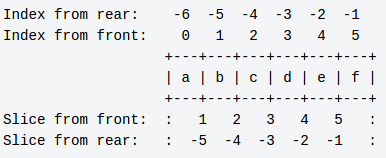
\includegraphics[width=\textwidth]{04_Data_Structures/indexing.png}

	\begin{center}
		
		\texttt{[a, b, c, d, e, f]}

	\end{center}

\end{frame}


\begin{frame}[fragile]{Iterating over Lists}
        \begin{pythoncode}
hp_list = ["harry", "ron", "hermione"]
print(len(hp_list)) # 3

# Iterating by index
for index in range(len(hp_list)):
    item = hp_list[index]
    # do something with item here
    print(item)

# Iterating by content
for item in hp_list:
    # do something with item here
    print(item)
        \end{pythoncode}


\end{frame}

\begin{frame}[fragile]{Nesting Lists}

        \begin{pythoncode}
def make_grid(height, width, value=1):
    grid = [] 
    for y in range(height):
        row = []
        for x in range(width):
           row.append(value)
        grid.append(row)
    return grid

my_grid = make_grid(3, 2)
print(my_grid) # ???

        \end{pythoncode}


\end{frame}

\begin{frame}[fragile]{Nesting Lists}

        \begin{pythoncode}
def make_grid(height, width, value=1):
    grid = []
    for y in range(height): # repeat for each row
        row = [] # create empty list
        for x in range(width): # repeat for each cell
           row.append(value) # add value to row
        grid.append(row) # add row to grid
    return grid	

my_grid = make_grid(3, 2)
print(my_grid) # [[1, 1], [1, 1], [1, 1]]

        \end{pythoncode}


\end{frame}

\begin{frame}[fragile]{Merging Lists}


    \begin{pythoncode}

list_a = [1, 2, 3]
list_b = ["cheese", "melon", "banana"]

merged = list_a + list_b
print(merged) # [1, 2, 3, "cheese", "melon", "banana"]

list_a.extend(list_b)
print(list_a) # [1, 2, 3, "cheese", "melon", "banana"]

	
	\end{pythoncode}


\end{frame}

\subsection{Evaluating Lists}

\begin{frame}{Evaluating Lists}

    \begin{enumerate}
		\item \texttt{len(list)}: Returns length of list
		\item \texttt{max(list)}: Returns maximum item of list
		\item \texttt{min(list)}: Returns minimum item of list
		\item \texttt{sum(list)}: Returns sum of items in list
		\item \texttt{sorted(list)}: Returns sorted copy of list
    \end{enumerate}

	\vspace{1em}
	How could we use these functions to calculate the average?

	\note{
	You never have to worry about implementing the most efficient sorting algorithm.
	The in-built functions sorted(), max() and min() implement Timsort in C, which is more efficient
	than anything you could implement on your own in pure Python.
	}

\end{frame}

\begin{frame}[fragile]{Evaluating Lists}

    \begin{pythoncode}

def average(any_list):
	return sum(any_list) / len(any_list)
    
my_list = [8, 2, 9, 3, 1]
print(len(my_list)) # 5
print(max(my_list)) # 9
print(min(my_list)) # 1
print(sum(my_list)) # 23 
print(sorted(my_list)) # [1, 2, 3, 8, 9]
print(average(my_list)) # 4.6

	\end{pythoncode}

\end{frame}

\section{More Data Structures}

\subsection{Tuples}

\begin{frame}[fragile]{Tuples}

    \begin{enumerate}
		\item Same as lists, but immutable (unchangeable)
		\item Creating: \texttt{my\_tuple = (v1, v2, v3)}
		\item Unpacking: \texttt{x1, x2, x3 = my\_tuple}
    \end{enumerate}

	\vspace{1em}

	\begin{pythoncode}
my_list = [1, 2, 3]
my_list[1] = 5
print(my_list) # [1, 5, 3]

my_tuple = (1, 2, 3)
my_tuple[1] = 5
# TypeError
	\end{pythoncode}


\end{frame}

\subsection{Sets}

\begin{frame}[fragile]{Sets}

    \begin{enumerate}
		\item Same as lists, but unique (duplicates automatically removed)
		\item Syntax: \texttt{s = \{v1, v2, v3\}}
		\item Not ordered (no indexing)
    \end{enumerate}

	\vspace{1em}

	\begin{pythoncode}
my_set = {1, 2, 2, 3}
print(my_set) # {1, 2, 3}
print(my_set[0])
# TypeError
	\end{pythoncode}

\end{frame}

\subsection{Dictionaries}

\begin{frame}[fragile]{Dictionaries}

    \begin{enumerate}
		\item Stores not only values, but also names ("keys")
		\item Creating: \texttt{my\_dict = \{key1: value1, key2: value\}}
		\item Indexing: \texttt{my\_dict[key1]}
		\item Keys must be immutable (e.g. Strings, Tuples)
    \end{enumerate}

	\vspace{1em}

	\begin{pythoncode}
my_dict = {"price_apples": 1.2, "price_banana": 4.8}
print(my_dict["price_apples"]) # 1.2
# Iterating by key value pairs
for key, value in my_dict.items():
	print(key, value)
	value = 7 # this will not change anything
	my_dict[key] = 29 # this will change something
print(my_dict) # {"price_apples": 29, "price_banana": 29}

	\end{pythoncode}

\end{frame}

\subsection*{General}

\begin{frame}{When to use which Data Structure?}

    \begin{enumerate}
		\item Lists         (ordered, mutable, all-purpose)
		\item Tuples        (ordered, immutable)
		\item Sets          (unordered, mutable, unique)
		\item Dictionaries  (unordered, mutable, custom-index)
    \end{enumerate}

\end{frame}

\section{Organisational}

\begin{frame}{Organisational}

    \begin{enumerate}
		\item In case of difficulties: Come to practice and feedback sessions!
		\item This week's exercise sheet will be \textbf{due Sunday 28th April 23:59 as usual}
		\item No lecture next week, but bonus exercise sheet
		\item Short survey regarding your current state of learning
    \end{enumerate}

\end{frame}

\begin{frame}{Organisational}

	\begin{center}

		
\includegraphics[width=0.5\textwidth]{04_Data_Structures/qr.png}
	
		\vspace{1em}

		\texttt{https://pingo.coactum.de/717836}

	\end{center}

\end{frame}


\end{document}
